\documentclass[10pt]{article}
\usepackage{icmlko}

\icmlmeta{IP 파운데이션 월드모델}{143}{대조군을 세우니 내 검정이 무너졌다}{노트 142가 만든 나이 검정을 날카롭게 하려다 그 검정의 기제 가설을 반증했다 --- 하루 만에}

\begin{document}

\twocolumn[
\icmlheader

\begin{abstract}
노트 142가 ``나이 검정''을 내놓았다 --- 설명문이 고정이면 작품 나이와 상관
세기가 무관해야 하고, 갱신되면 오래된 쪽이 세진다. 모바일만 걸렸고
($+$0.095) 그것으로 모바일의 글·그림 축을 사후로 등록했다. 그 노트가
남긴 첫 줄이 ``라벨 누적 효과와 안 갈린다 --- 상한이다''였다. 갈라 봤다.
\textbf{대조군을 세우면 갈린다} --- 라벨 잡음은 모든 축에 똑같이 걸리고
설명문 갱신은 글·그림 축에만 걸리므로, 이중차분이 남는다. 결과가 둘
바뀌었다. 모바일의 $+$0.095가 \textbf{$+$0.059}로 줄었고(37\%가 라벨 잡음),
\textbf{게임이 새로 걸렸다}($+$0.082 --- 원값은 $+$0.017인데 대조가
$-$0.065다). \textbf{그리고 직접 검정을 했다.} 모바일 레코드에는
\texttt{updated} 필드가 있다 --- 출시일과 최종 갱신일의 간격이 크면 설명이
많이 바뀐 것이다. 무통제로 재니 갱신 간격이 큰 쪽의 $|\rho|$가 0.217로
작은 쪽 0.150보다 세다($+$0.067). \textbf{가설과 맞고 이중차분과도
가깝다.} 그런데 출시 연도를 고정하고 다시 재니 \textbf{부호가 뒤집힌다}
--- 0.216 대 0.145로 갱신 간격이 큰 쪽이 \emph{약하고}, 다섯 연도 밴드가
전부 같은 방향이다. \textbf{무통제 $+$0.067은 전부 나이 교란이었다.}
그러므로 노트 142의 나이 검정은 사후 탐지기로 검증되지 않았다. 모바일의
나이차는 실재하지만 기제가 설명문 갱신은 아니다. 등록부의 모바일 차단은
남긴다 --- 노트 141의 ``모르면 막는다''에 따르고, 그 비용이 판 $+$0.006
뿐이다.
\end{abstract}
]

\begin{figure*}[t]
\centering
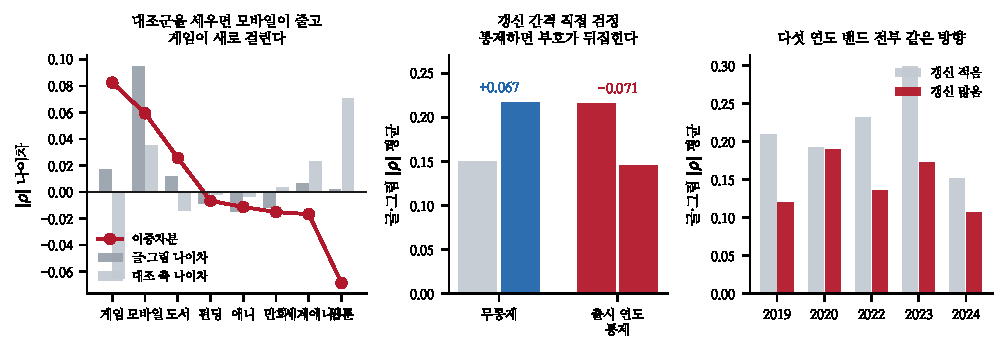
\includegraphics[width=\textwidth]{figs/did.pdf}
\caption{왼쪽 --- 이중차분. 가운데 --- 갱신 간격 직접 검정, 통제하면 부호가
뒤집힌다. 오른쪽 --- 다섯 연도 밴드 전부 같은 방향.}
\end{figure*}

\section{대조군을 세우면 갈린다}

노트 142의 나이 검정에는 알려진 구멍이 있었다. 오래된 작품은 라벨이 더
쌓여 잡음이 적으므로, 갱신이 없어도 오래된 쪽에서 상관이 세게 나온다.
그 노트에 ``상한이다''라고 적어 두었다.

가르는 방법이 있다. \textbf{라벨 잡음은 모든 축에 똑같이 걸리고, 설명문
갱신은 글·그림 축에만 걸린다.} 그러니 사전 축(손 축 다섯 · 검색 · 달력)의
나이차를 빼면 갱신 몫만 남는다.

\begin{table}[t]
\centering\tsize
\caption{$|\rho|$ 나이차. 후행을 나이로 반 갈랐다.}
\begin{tabular}{lrrr}
\toprule
& 글·그림 & 대조 축 & 이중차분 \\
\midrule
\textbf{게임} & $+$.017 & $-$.065 & \textbf{$+$.082} \\
\textbf{모바일} & $+$.095 & $+$.035 & \textbf{$+$.059} \\
도서 & $+$.011 & $-$.014 & $+$.026 \\
펀딩 & $-$.008 & $-$.002 & $-$.007 \\
애니 & $-$.015 & $-$.004 & $-$.011 \\
만화 & $-$.012 & $+$.004 & $-$.015 \\
세계애니 & $+$.007 & $+$.023 & $-$.017 \\
웹툰 & $+$.002 & $+$.070 & $-$.069 \\
\bottomrule
\end{tabular}
\end{table}

\claimx{\textbf{모바일이 줄고 게임이 새로 걸린다.} 모바일의 $+$0.095 중
37\%가 라벨 잡음이었다. 게임은 원값이 $+$0.017로 작은데 대조가 $-$0.065라
이중차분이 $+$0.082다.}{게임의 신호는 \emph{대조가 움직여서} 생긴 것이다
--- 글·그림은 거의 평평하다. 이중차분은 ``갱신이 없으면 두 쪽 나이차가
같다''를 전제하는데 그 전제는 검정 안 했다.}

\section{그래서 직접 쟀다}

모바일 레코드에 \texttt{updated}가 있다. 출시일과 최종 갱신일의 간격이
크면 설명이 그만큼 바뀐 것이다. 가설이 맞다면 간격이 큰 쪽에서 글·그림
상관이 세야 한다.

\begin{table}[t]
\centering\tsize
\caption{모바일. 글·그림 축 스무 개 $|\rho|$ 평균.}
\begin{tabular}{lrrr}
\toprule
& 갱신 적음 & 갱신 많음 & 차 \\
\midrule
무통제 & .150 & .217 & \textbf{$+$.067} \\
\textbf{출시 연도 통제} & .216 & .145 & \textbf{$-$.071} \\
\bottomrule
\end{tabular}
\end{table}

\claimx{\textbf{무통제로는 가설과 맞는다} --- $+$0.067이고 이중차분 추정
$+$0.059와 가깝다. 두 경로가 같은 값을 낸다.}{여기서 멈추면 ``두 방법이
서로를 뒷받침한다''로 읽힌다. 실제로 그렇게 읽을 뻔했다.}

\claimx{\textbf{출시 연도를 고정하면 부호가 뒤집힌다.} 갱신 간격이 큰
쪽이 0.145로 작은 쪽 0.216보다 \emph{약하다}. 다섯 연도 밴드에서 전부
같은 방향이다($-$0.002 $\sim$ $-$0.126). \textbf{무통제 $+$0.067은 전부
나이 교란이었다} --- 오래된 앱일수록 갱신 간격도 크고 라벨도 성숙하다.}{``간격''이
갱신 \emph{횟수}나 내용 변화량은 아니다. 어제 한 번 갱신한 오래된 앱도
간격이 크다. 검정이 완벽하지는 않다.}

\section{그러면 나이 검정은 무엇인가}

\claimx{\textbf{사후 탐지기로 검증되지 않았다.} 모바일의 나이차는 실재하지만
(이중차분 $+$0.059) 기제가 설명문 갱신이라는 증거는 직접 검정에서
무너졌다. 나이차에는 라벨 성숙이라는 무해한 설명이 있고, 이중차분의
평행추세 전제는 검정 안 됐다.}{노트 142가 나이 검정을 ``등록부가 빠뜨린
것을 자료로 잡는 방법''이라고 적었는데, 그만큼의 지위는 아직 없다.
\textbf{기제를 짚지 못하는 탐지기는 경고지 판정이 아니다.}}

등록부의 모바일 차단은 남긴다. 근거는 세 가지다. 노트 141이 세운 ``모르면
막는다''에 따르고, 앱스토어 목록이 갱신된다는 것은 자료 밖의 상식이며,
막는 비용이 판 $+$0.006뿐이다.

\begin{table}[t]
\centering\tsize
\caption{같은 자료를 세 방법으로 재면.}
\begin{tabular}{lrl}
\toprule
& 값 & 판정 \\
\midrule
나이 검정 (노트 142) & $+$.095 & 갱신 의심 \\
이중차분 (노트 143) & $+$.059 & 갱신 의심 \\
갱신 간격 · 무통제 & $+$.067 & 갱신 의심 \\
\textbf{갱신 간격 · 연도 통제} & \textbf{$-$.071} & \textbf{반증} \\
\bottomrule
\end{tabular}
\end{table}

세 방법이 같은 방향을 가리키고 네 번째가 뒤집었다. \textbf{여러 방법이
일치하는 것이 옳음의 증거가 아니다} --- 셋이 같은 교란을 공유하고 있었다.

\begin{table}[t]
\centering\tsize
\caption{남은 것.}
\begin{tabular}{ll}
\toprule
게임 & 이중차분만 걸렸다 --- 직접 검정할 자료가 없다 \\
평행추세 & 이중차분의 전제를 검정할 방법 \\
등록부 & 자료로 검증 못 하면 상식에 기댄다 --- 명시할 것 \\
\bottomrule
\end{tabular}
\end{table}

마지막 줄을 등록부에 적어 두기로 한다. 지금 \texttt{provenance.py}의
분류에는 ``자료로 확인함''과 ``상식으로 판단함''이 섞여 있는데, 노트 141과
142와 143이 보여 준 대로 그 둘은 무게가 다르다.

\end{document}
